%!TEX root = ../aamas11storage.tex
%%%%%%%%%%%%%%%%%%%%%%%%%%%%%%%%%%%%%%%%%%%%%%%%%%%%
\section{An Energy Storage Application}\label{sec:application}
%%%%%%%%%%%%%%%%%%%%%%%%%%%%%%%%%%%%%%%%%%%%%%%%%%%%



Energy storage enables increasing levels of renewable energy in our electricity system, and the rapidly maturing supply chains for several battery technologies encourages electricity utilities, generators, and customers to consider using large battery systems. 
Consider a controller for managing the overall energy demand of a smart office building comprising of a set of loads (e.g., appliances in the building), some renewable sources (e.g., solar panels on the roof and a local wind turbine), and a \emph{modular battery system}. The building is connected to the main electricity grid, and economics govern that the overall grid power demand of the building be maintained within the range $[0:p_h]$; see Figure~\ref{fig:usecase}. 
%%
Since there is little control over the demand in the building, and certainly no control over the renewable generation, it is possible that the building power consumption falls outside this range for some period in the day. For instance, if the renewable generation is high relative to the building loads, then net consumption (Building Demand) may fall below $0$ (e.g., period prior to $t_1$); whereas if demand is higher than generation, then the net building consumption may rise above $p_h$ (e.g., period after $t_2$). 
%
%While net demand is fixed for all practical purposes, 
While there is little that can be done about the net building consumption and generation,
we do have control over the use of the battery system. Hence, by suitably ordering the battery system (Battery Charge) to charge (i.e., act as a load) or discharge (i.e., act as a generator) at determined rates, it is possible to influence the net demand and effectively the energy drawn from the electricity grid (Grid Supply).
%%

Large battery systems usually comprise of multiple modules that can be controlled independently~\cite{norris02:grid}.  Modules may be operated in synchrony, but there are often strategic reasons for keeping some modules in different states.  For example, if it is undesirable to change the direction of power flow between charging and discharging too frequently, a subset of modules may be used for each direction until it is necessary to swap their roles. Also, some technologies have specific requirements, such as zinc-bromine flow batteries needing complete discharges at regular intervals to ``strip'' the zinc plating and hence ensuring irregularities never accumulate. Where they exist, such requirements place further constraints on module control.

So, given a large battery installation, we are interested in a mechanism to achieve a desired rate of charging or discharging, by suitably setting each module in the battery---the overall rate being the sum over the modules' rates.  
%%
For simplicity, we assume homogeneous capacity $c$ of the modules (but with possibly different chemical properties and constraints), and hence an overall system capacity of $c \times k$ (where $k$ is the total number of modules in the system). Each module, in turn, may be configured as charging ($+c$), discharging ($-c$), or not in use ($0$). By appropriately setting each module's operational state, the total response of the battery system may be adjusted in steps of $\pm c$.
%%
While hardwired control is indeed possible, it is not ideal due to the fact that battery performance is susceptible to changes over time---modules tend to lose actual capacity---and may diverge from normal. 
%%
What is required is an \emph{adaptable} control mechanism that accounts for such drift. 
%%

Figure~\ref{fig:gptree} depicts a BDI controller for this application. Top-level goal-event $G(r,k,s)$ requests a battery charge/discharge (normalized) rate of $r \in [-1.0:+1.0]$, where $-1.0$ ($1.0$) indicates maximum discharge (charge) rate, $s$ stands for the current state of the battery system as per sensor readings, and $k$ is (initially) the number of modules in the system. 
%%
The BDI controller works by recursively configuring each module for the period in question using the plans $\pSetCharge$ (charging at rate $+c$), $\pSetDischarge$ (discharging at rate $-c$), and $\pSetNotUsed$ (disconnected), and finally, after all modules have been configured, physically operating the battery for one period using the $\pExecute$ plan. 
%%

Observe that the first three plans already contain initial known (necessary) domain constraints for applicability, by means of conditions $\cSatisfies_X(\cdot,\cdot,\cdot)$. For instance, plan $\pSetCharge$ may not be considered in a given instance if the module is only allowed to change charge directions once every four periods and charging in this period would violate this constraint. 
Similarly, plan $\pSetDischarge$ may be ruled out because discharging the module implies that regardless of how the remaining modules are configured, the response is bound to fall short of the request.
When none of the first three plans apply for a given module, then BDI failure recovery may be employed to backtrack up and select a different configuration path until all constraints are satisfied (or all options are exhausted). 

As such, the $\pExecute$ plan is run only with configurations that are functionally correct.
%
When this happens, the whole battery system is first executed for the period (action $\aOperate$) and its performance evaluated via a sensor (action $\aEvaluate$). If the evaluation step \emph{succeeds}, then the desired overall rate $r$ has been met and the whole execution is assumed successful. If, on the other hand, the desired overall rate has not been met in reality, the evaluation step \emph{fails} and so does the whole execution of the program, since no BDI failure recovery can be used after the battery system has been physically operated. 












%%%%%%%%%%%%%%%%%%%%%%%%%%%%%%%%%%%%%%%%%%%%%%%%%%%%%
%\section{Modular Battery Controller}\label{sec:introduction}
%%%%%%%%%%%%%%%%%%%%%%%%%%%%%%%%%%%%%%%%%%%%%%%%%%%%%
%Energy storage enables increasing levels of renewable energy in our electricity system, and the rapidly maturing supply chains for several battery technologies encourages electricity utilities, generators, and customers to consider using large battery systems. 
%
%Consider the example scenario of a smart office building comprising of a set of loads (appliances in the building), some renewable sources (solar panels on the roof and a local wind turbine), and a modular battery system. The building is connected to the main grid, and economics govern that the grid power consumption of the building be maintained within the range $[0:p_h]$. Since there is little control over the demand in the building and certainly no control over the renewable generation, then for some period in the day it is possible that the power consumption of the building will fall outside this range. For instance, if the renewable generation is high relative to the building loads, then net consumption may fall below $0$. Similarly, if demand is higher than generation then the net building consumption may rise above $p_h$. In Figure \ref{fig:usecase} the Building Demand curve for the period prior to $t_1$ and after $t_2$, has this property. While this net demand is fixed for all practical purposes, we do have control over the use of the battery system. By suitably ordering the battery system to charge (act as a load) or discharge (act as a generator) at determined rates through this period we may influence the net demand in the building. Figure \ref{fig:usecase} shows how the appropriate battery response (Battery Charge) added to the net building consumption (Building Demand) ensures that the power drawn from the grid (Grid Supply) is maintained within the desired range.
%
%\begin{figure}[ht]
%\begin{center}
%%!TEX root = ../aamas11storage.tex
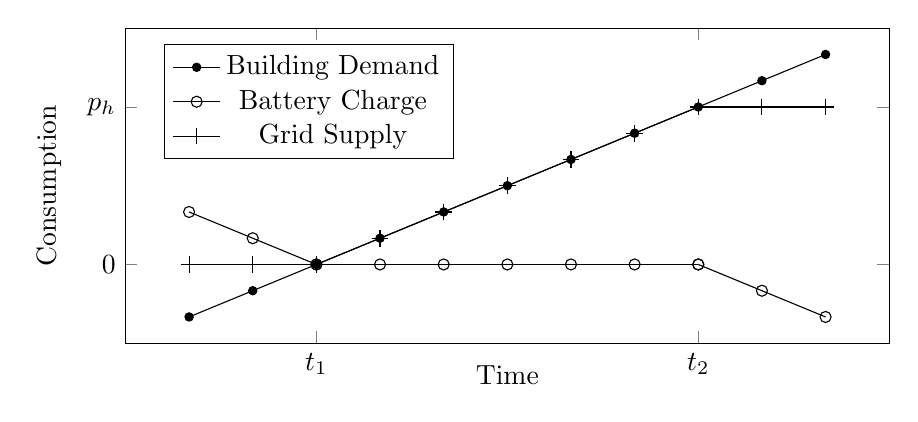
\begin{tikzpicture}

\begin{axis}[
width=0.8\columnwidth,height=4cm,scale only axis,
axis line style={-}, xtick style={-}, ytick style={-},
xlabel=Time,
ylabel=Consumption,
every axis y label/.style={at={(-0.1,0.5)},rotate=90,anchor=center}, 
every axis x label/.style={at={(0.5,-0.1)},anchor=center}, 
%grid=both, grid style={style=densely dotted},
xtick={2,8},
xticklabels={$t_1$,$t_2$},
ytick={0,6},
yticklabels={$0$,$p_h$},
legend style={at={(0.05,0.95)},anchor=north west}
] 

% Draw the Demand-Supply curve
\addplot[-,mark=*,mark size=1.5] expression[domain=0:10,samples=11] {x-2};
\addlegendentry{Building Demand} 

% Draw the Battery curve
\addplot[-,mark=o,mark size=2] expression[forget plot,domain=0:2,samples=3] {2-x}; 
\addplot[-,mark=o,mark size=2] expression[forget plot,domain=2:8,samples=7] {0}; 
\addplot[-,mark=o,mark size=2] expression[domain=8:10,samples=3] {8-x}; 
\addlegendentry{Battery Charge} 

% Draw the Grid supply curve
\addplot[-,mark=+,mark size=3] expression[forget plot,domain=0:2,samples=3] {0}; 
\addplot[-,mark=+,mark size=3] expression[forget plot,domain=2:8,samples=7] {x-2}; 
\addplot[-,mark=+,mark size=3] expression[domain=8:10,samples=3] {6}; 
\addlegendentry{Grid Supply} 
\end{axis} 
\end{tikzpicture} 

%\end{center}
%\caption{Use case scenario for a modular battery system.}
%\label{fig:usecase}
%\end{figure}
%
%Large battery systems usually comprise of multiple modules and in many installations these may be controlled independently.  Modules may be operated in synchrony but often there are strategic reasons to keep some modules in a different state to others.  For example, if it is undesirable to change the direction of power flow between charging and discharging too frequently, a subset of modules may be used for each direction until it is necessary to change their roles.  Also, some technologies have specific requirements, such as the zinc-bromine flow battery for which a complete discharge at regular intervals is desirable to ``strip'' the zinc plating and ensure irregularities never have an opportunity to accumulate.  Where they exist these requirements place further constraints on module control.
%
%Given, then, a requested rate of charging and discharging for a large battery installation, we would like a control algorithm for the set of component modules that implements the requested rate as the sum over the module rates of charging and discharging.  While hardwired control of such response is possible, it is not ideal since battery performance is susceptible to change over time and may diverge from normal. What is required is a means of adaptable control that accounts for such drift, and as such, a machine learning approach may be appropriate. 
%%The input signal will be different every day but will have many features that are diurnal or nearly so, due to typical variations of electricity demand and solar and wind energy generation sources, and the repetitive patterns that may be seen over several days of the input signal suggest that a learning algorithm may be appropriate.  Our problem is to develop a method for on-line learning that will result in a useful control regime for a modular battery system, when installed at a new site and provided with an input signal derived from the electricity demand and renewable supply at that site.
%
%\begin{figure*}[ht]
%\begin{center}
%%!TEX root = ../aamas11storage.tex
\begin{tikzpicture} [level distance=8.0em]
\tikzstyle{planbox}=[draw,text width=11.0em,rectangle split,rectangle split parts=3]
\tikzstyle{goalbox}=[draw,rounded corners=1.25em,minimum height=3em,minimum width=5em]

	
\tikzstyle{level 1}=[sibling distance=13.0em] 
\tikzstyle{level 2}=[level distance=7.0em] 

\node[goalbox,solid] {$G($r,k,s$)$}
	child {node[planbox] {$SetCharge$ 
			\nodepart{second} $\psi:satisfies(r,k,s,C),$\\$k>0$
			\nodepart{third} $set(k,C)$
		}
		child {node[goalbox] {$G($r,k-1,s'$)$}}
	}
	child {node[planbox] {$SetDischarge$ \nodepart{second}
			\nodepart{second} $\psi:satisfies(r,k,s,D),$\\$k>0$
			\nodepart{third} $set(k,D)$
		}
		child {node[goalbox] {$G($r,k-1,s'$)$}}
	}
	child {node[planbox] {$SetNotUsed$ \nodepart{second}
			\nodepart{second} $\psi:satisfies(r,k,s,N),$\\$k>0$
			\nodepart{third} $set(k,N)$
		}
		child {node[goalbox] {$G($r,k-1,s'$)$}}
	}
	child {node[planbox] {$Execute$ 
			\nodepart{second} $\psi:k==0$
			\nodepart{third} $operate()$ \\$evaluate()$
		}
	}
;

\end{tikzpicture}



%\end{center}
%\caption{Goal-plan hierarchy for the battery system with $k$ modules.}
%\label{fig:gptree}
%\end{figure*}
%
%
%%%%%%%%%%%%%%%%%%%%%%%%%%%%%%%%%%%%%%%%%%%%%%%%%%%%%
%\subsection{System Design}\label{subsec:design}
%%%%%%%%%%%%%%%%%%%%%%%%%%%%%%%%%%%%%%%%%%%%%%%%%%%%%
%
%Figure \ref{fig:gptree} shows a BDI controller for a battery system with $k$ modules. At the beginning of each period of deliberation, the environment posts the top-level goal $G(r,k,s)$. The controller responds by operating the battery system for that period in a suitable operational state that resolves the goal. Here $r$ specifies the desired response from the battery system and lies in the normalised range $[-1.0:+1.0]$ where $-1.0$ indicates a maximum discharge rate (where all modules are discharging) and $+1.0$ indicates a maximum charge rate (where all modules are charging). The parameter $s$ represents the current state of the battery system derived from sensor readings, and $k$ is initially set to the number of modules in the system. 
%
%The resolution of the battery system decides how closely it can match the desired response and is determined by the number of modules $n$. For simplicity, we will assume homogeneous capacity of the modules (but with possibly different chemical properties and constraints), such that each module has a normalised capacity $c$ and $c*n=1.0$. Each module in turn may be configured in one of three states: charging (i.e $+c$), discharging (i.e. $-c$) or not in use (i.e. $0$). The sum of these values gives the net response of the system. By appropriately setting each module's operational state then, the response of the battery system may be adjusted in the range $[-1.0:+1.0]$ in steps of $\pm c$.
%
%The BDI controller works by recursively configuring each module using the respective $Set*$ plans, and then finally operating the battery for one period using the $Execute$ plan. The {\em active execution trace} therefore always consists of the selection of $k$ high level $Set*$ plans followed by the selection of the $Execute$ leaf plan. 
%
%The plans in the hierarchy are further explained below:
%
%$SetCharge$: Set the configuration of module $k$ to {\em charging} (i.e $+c$) for this period. The plan's context condition first checks that the internal constraints of module $k>0$ will not be violated by this operation. If the context condition fails then the plan is discarded, otherwise the configuration is updated and Goal $G$ reposted for module $k-1$.
%
%$SetDischarge$: Set the configuration of module $k$ to {\em discharging} (i.e $-c$) for this period. The plan's context condition first checks that the internal constraints of module $k>0$ will not be violated by this operation. If the context condition fails then the plan is discarded, otherwise the configuration is updated and Goal $G$ reposted for module $k-1$.
%
%$SetNotUsed$: Set the configuration of module $k$ to {\em not in use} (i.e $0$). This means that the module will remain disconnected from use for this period. The plan's context condition first checks that the internal constraints of module $k>0$ will not be violated by this operation. If the context condition fails then the plan is discarded, otherwise the configuration is updated and Goal $G$ reposted for module $k-1$.
%
%$Execute$: Leaf plan to physically operate the battery system. The plan executes only when $k=0$ which implies that all modules have been configured. The battery modules are then operated simultaneously for one period according to their assigned configurations. 
%
%$Set*$ plans are discarded from consideration when their context condition does not hold for that period. For instance, plan $SetCharge$ may be discarded because module $k$ is only allowed to change charge directions once every four periods say, and charging it in this period will violate that constraint. Similarly, plan $SetDischarge$ may be discarded because the module may already be discharged and further discharge is not possible. 
%
%Since such constraint checking is performed in the context condition of the plans prior to physical operation of the battery, then BDI failure recovery may be employed to select different $Set*$ plans until all internal constraints are satisfied. Note that failure recovery is not allowed for the $Execute$ plan because it runs for a full period and that is the limit for the decision making. In other words, only one try (in terms of physically operating the battery) is allowed per period.
%
%Finally, the context condition of the $Set*$ plans performs {\em operational constraint checking} to decide if the configuration is admissible for module $k$: given the desired response $r$, the modules configured to so far i.e $[0 \ldots k-1]$, and the number of modules yet to be configured i.e $[k+1 \ldots n]$. For instance, a request of $+1.0$ is only serviceable when all modules are configured to charge. So, if module $k$ were to not charge (it may already be fully charged so further charging is not possible), then the operational constraint for module $k+1$ will fail because the ``bad'' configuration of module $k$ implies that regardless of how the remaining modules are configured, the response is bound to fall short of the request. When this happens, BDI failure recovery allows us to backtrack up the chain of active $Set*$ plans and choose a different path until all constraints are met. As such, the $Execute$ plan is run only with configurations that are functionally correct.
%